\label{sec:uq_overview}

The Uncertainty Quantification (UQ) module of FOQUS provides a multitude of analysis and visualization
capabilities to facilitate the understanding of uncertainty's impact on a
given system. In a generic UQ study, the workflow is usually comprised of the following
steps:

\begin{enumerate}
	\item Define the objectives of the analysis.
	\item Specify and acquire the simulation model, which implements an
     input-to-output mapping from inputs to outputs.
	\item Select the inputs that have uncertainty and characterize said
     uncertainty in the form of \emph{prior} distributions.
	\item Identify relevant data from physical experiments that can be used
     to refine these prior distributions on the inputs.
	\item Generate a set of input samples according to the input
     distribution.
	\item Propagate the set of input samples through the simulation model to 
     get the corresponding output values.
	\item Analyze the results to make informed decisions about subsequent analyses.
\end{enumerate}
FOQUS UQ provides tools to perform Steps 5-7. With respect to Step 7, a
variety of analysis capabilities are available. They include parameter
screening methods, response surface construction/validation/prediction,
uncertainty analysis, sensitivity analysis, and visualization.

In this chapter, components of the UQ user interface are first explained,
then the use of these components for UQ analyses is illustrated.

\section{UQ User Interface}

The UQ module enables the user to perform UQ studies on a flowsheet. 
From the Uncertainty button on the Home window, the user can configure different simulation ensembles
(different sets of samples generated using different sampling schemes), run
them, and perform analyses. This screen is illustrated in Figure
\ref{fig:uq_screen}.

%%% INSERT: UQ Screen
\begin{figure}[H]
\centering 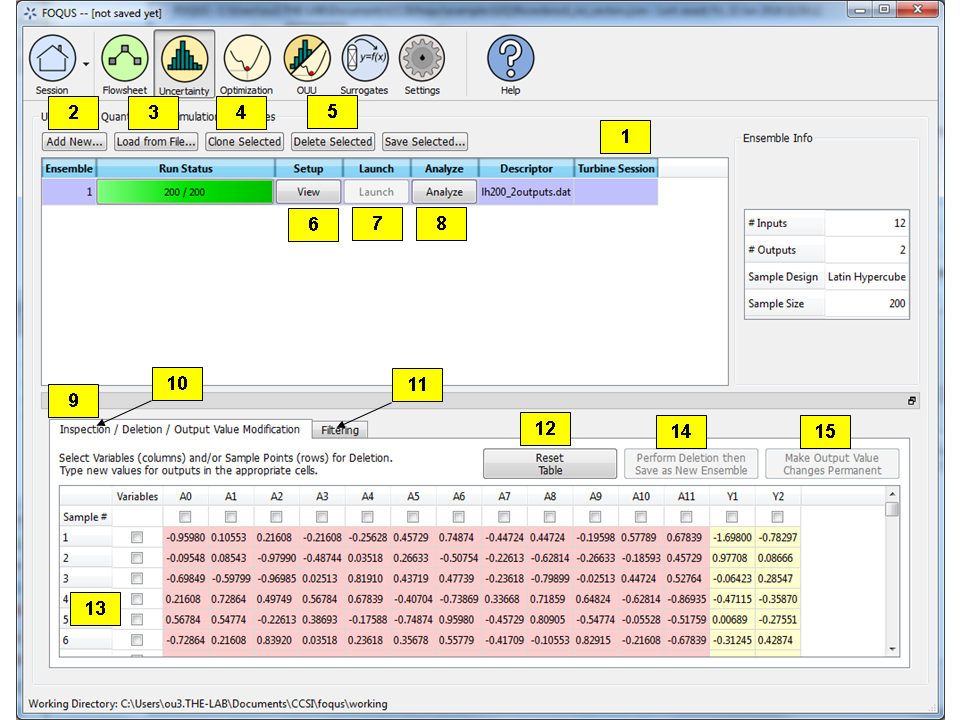
\includegraphics[width=6.5in,height=4in,keepaspectratio]{Chapt_uq/figs/overview/1_UQScreen2}
\caption{Uncertainty Quantification Screen}
\label{fig:uq_screen}
\end{figure}
\begin{enumerate}
\item
	\bu{Simulation Ensemble Table} displays all of the simulation ensembles:
	each ensemble being a row in the table. A simulation ensemble is a
	collection of sample points where each sample point has a different set
	of values for the uncertain variables. The values of these variables are
	generated based on the sampling scheme designated by the user. When
	launched, the output values of the sample points are calculated based on
	the generated sample input values. Subsequently, the corresponding
	simulation outputs can be analyzed. For each ensemble, the table
	displays the \textbf{\underline{Ensemble}} index, \textbf{\underline{Run Status}} (how many have been
	completed), \bu{Setup} and \bu{Launch} options (discussed below), and a
	\textbf{\underline{Descriptor}}. The \textbf{\underline{Descriptor}} contains the name of the corresponding node
	in the flowsheet or the name of the file if the ensemble was loaded from
	a file. Additional sample information such as \textbf{\underline{\# Inputs}}, \textbf{\underline{\# Outputs}}, \textbf{\underline{Sample Design}}, and \textbf{\underline{Sample Size}} are also displayed on
	the right.
\item 
	\bu{Add New} creates a simulation ensemble (a set of input samples)
	as a new row in the \bu{Simulation Ensemble Table}. Once clicked, a
	dialog is displayed to prompt the user to choose between using (1) a
	flowsheet (an exact simulation model) or (2) a response surface (an
	approximate simulation model or an emulator) associated with the
	ensemble. \\
	If using an emulator, the user must browse a PSUADE-formatted file that
	contains the training data for the emulator (in this version, the
	response surface type has been designated inside the sample file and can
	only be changed by editing the sample file) and select the output(s) to
	be evaluated by the trained emulator. Subsequently, a simulation setup
	dialog box is displayed for setting up the distributions of input
	variables and the sampling scheme to generate samples of the uncertain
	input variables. This \textbf{\underline{Simulation Ensemble Setup}} dialog is explained in further detail in Section \ref{subsec:uq_simsetup}.
\item
	\bu{Load from File} loads a simulation ensemble from a sample file
 	that conforms to the PSUADE full file format. (See
 	Section \ref{ap:psuadefiles} for details on the PSUADE full file format.)
   The user can click \bu{Save Selected} to save an existing ensemble as a
 	PSUADE full file, and load it by clicking \bu{Load from File} to perform
 	further analyses. 
\item
	\bu{Clone Selected} clones the selected simulation ensemble and adds the
	copy as a new row at the end of the table. This ensemble can then be
	edited (e.g., depending on whether the ensemble has been run, the user
	has different options for modifying the ensemble). 
   This allows the user to create a new ensemble similar to
	the current ensemble without having to start from scratch (i.e., setting
	up the input parameters). For example: (1) \bu{Clone Selected} can be used in
	conjunction with \bu{Load from File} to clone an existing ensemble
	before input/output modification to prepare a new but similar
	ensemble for UQ analysis. (2) \bu{Clone Selected} can also be used to
	prepare a fresh ensemble for evaluation via a different simulation
	model. In this case, the user should save the cloned ensemble,
	reload it by clicking \bu{Add New}, associate it with a node, and then
	click \textbf{\underline{Launch}} to start the runs. 
\item
	\bu{Delete Selected} deletes the currently selected simulation ensemble.
\item
	\bu{Revise} enables a user to change a simulation ensemble before launching
	the run. If the ensemble was previously run or it is cloned from an
	already-generated sample, the corresponding button becomes \bu{View} so
	the user can view the input samples in the simulation ensemble. 
\item
	\bu{Launch} starts the simulation process of the ensemble. (\bu{Launch}
	is not enabled until the user has setup everything needed for
	simulations.) A simulation is launched for each sample point to compute
	the corresponding outputs.
\item
	\bu{Analyze}, when enabled (after all simulation results are ready),
   enables the user to perform various UQ analysis to the ensemble.  When
   clicked, a new dialog box displays, allowing the user to configure and
   run analysis.
\item
	\bu{Data Manipulation} enables (1) the deletion of inputs, outputs, or samples, 
	(2) the	modification of output values for specific sample points, and 
	(3) the range-based filtering of samples.
\item
	\bu{Inspection/Deletion/Output Value Modification} serves three purposes: 
	it enables the user to (1) view the numerical values of samples in table form, 
	(2) delete variables and/or samples, and (3) edit the output values of 
	specific samples. \textbf{\underline{Deletion}} creates a new simulation	ensemble as a new 
	row in the simulation table that contains only those inputs/outputs and 
	samples that were not selected for deletion. \textbf{\underline{Output Value Modification}} 
	changes the values within the ensemble itself.
\item
	\bu{Filtering} enables the user to filter samples based on the values of
	an input or output. First, select the ensemble to be filtered from the \textbf{\underline{Simulation Ensemble Table}}. Once filtering is complete, a new simulation ensemble is
	added as a new row in the simulation table. The new simulation ensemble
	contains only those samples that satisfy the filtering criterion (with
	input or output samples within the specified range).

\item
	\bu{Reset Table} resets the table to default, meaning all variable and
	sample selections are unselected and output values within
	the table are reverted back to their original values, thus undoing any
	edits to the table.
\item
	The table displays the values of inputs	and outputs for each sample. 
	Inputs are highlighted in pink; outputs are highlighted in yellow. The user can select which 
	variables (columns) to delete by selecting the checkboxes on top. Likewise, 
	the user can select which samples (rows) to delete by selecting the checkboxes 
	on the left. Multiple samples can also be selected/deselected by using 
	(1) Shift+Click or Ctrl+Click to select multiple rows, or (2)
	right-clicking to bring up a menu to check or uncheck the checkboxes
	corresponding to the rows of the selected samples. In addition, 
	the user can change any output value by editing the appropriate cell. These 
	modified cells are highlighted green until changes are made permanent by clicking the
	appropriate button.
\item
	\bu{Perform Deletion then Save as New Ensemble} creates a new simulation
	ensemble as a new row in the \textbf{\underline{Simulation Ensemble Table}}. The new ensemble
	is without the variables and samples that were previously selected for
	removal.
\item
	\bu{Make Output Value Changes Permanent} overwrites the output values in
	the current ensemble with those that are highlighted green in the table.

\suspend{enumerate}

The \bu{Filtering} tab is illustrated in
Figure \ref{fig:uq_deltab} and enables the user to filter samples based on the values 
of an input or output.
%%% INSERT Filtering Tab 
\begin{figure}[H]
\centering \includegraphics[width=6.5in,height=4in,keepaspectratio]{Chapt_uq/figs/overview/2_FilteringTab2}
\caption{Filtering Tab} 
\label{fig:uq_deltab}
\end{figure}

\resume{enumerate}
\item
	\bu{Filter Input} filters based on the value of a certain input. Select
	an input variable as the filter target, and enter the lower and upper
	thresholds to specify a range of values to be kept in the new ensemble.
\item
	\bu{Filter Output} filters based on the value of a certain
	output. Select an output variable as the filter target, and enter the
	lower and upper thresholds to specify a range of values to be kept in
	the new ensemble.
\item
	Once the filter settings are set,
	click \bu{Perform Filtering then Save as New Ensemble} to apply the
	filter and create a new simulation ensemble.
\suspend{enumerate}

The single-output \textbf{\underline{Analysis of Ensemble}} dialog, which is displayed when \bu{Analyze}
is clicked for the selected ensemble, has two modes, as shown in
Figure \ref{fig:uq_analysisW} and Figure \ref{fig:uqt_rsaeua}.  
%%% INSERT Single-Output Analysis Section, Wizard Mode
\begin{figure}[!htb]
\centering 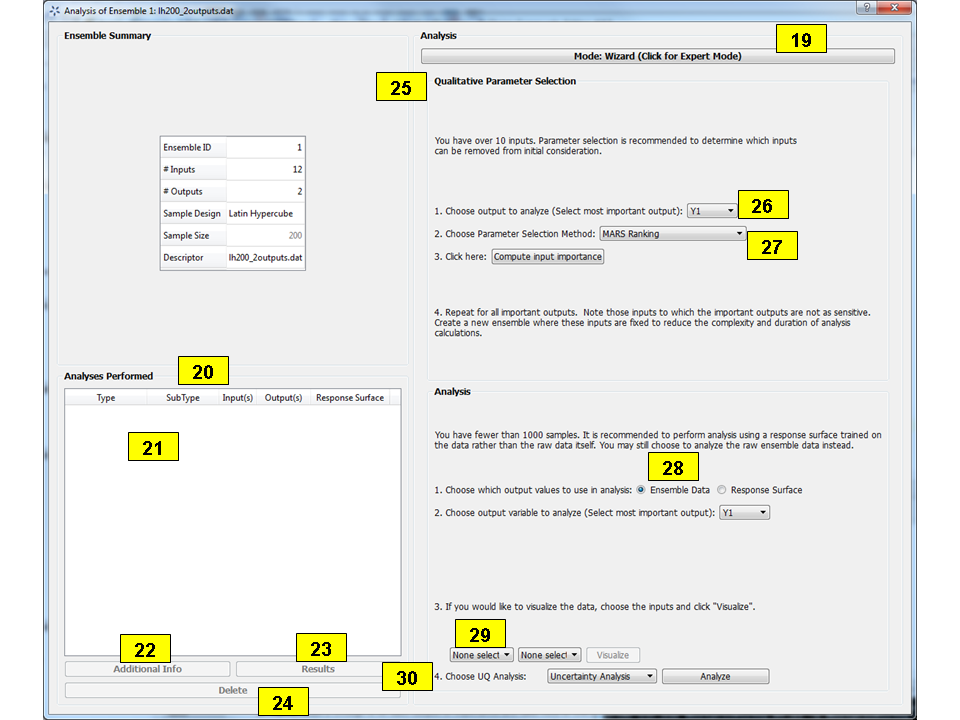
\includegraphics[width=6.5in,height=4in,keepaspectratio]{Chapt_uq/figs/overview/3_AnalysisSection2}
\caption{Analysis Dialog, Ensemble Data Analysis, Wizard Mode}
\label{fig:uq_analysisW}
\end{figure}

\resume{enumerate}
\item
	Select \bu{Wizard} or \bu{Expert} mode. The \textbf{\underline{Wizard}} mode provides more
   detailed guidance on how to perform UQ analysis. For users familiar with
   UQ analysis techniques, the \textbf{\underline{Expert}} mode provides more functionality
   and flexibility but with less guidance on its use. For example,
   users will be able to customize the input distributions, as well as run
   more advanced uncertainty analysis that handles both epistemic and
   aleatory uncertainties.
\item
	The \bu{Analyses Performed} section provides the user a history of
	previous analyses that were performed. The results of these analyses are
	cached, so the user can plot the analysis results without having to
	recompute them. 
\item
	The \bu{Analysis Table} populates as the user performs analyses. It
	lists previous analyses that the user has performed, along with some 
	of the main analysis settings (analysis type, inputs and outputs analyzed,
	etc.)
\item
	Depending on the type of analysis performed, the \bu{Additional Info} button displays
	any additional settings or parameters set by the user in the selected
	analysis that were not shown in the \textbf{\underline{Analysis Table}}.
\item
	The \bu{Results} button will display the results of the selected
	analysis. 
\item
	The \bu{Delete} button will delete the selected analysis from the
   history of previous analyses.  Once deleted,
	the user will need to perform the analysis again to see its results.
\item
	The \bu{Qualitative Parameter Selection} (top part of the \textbf{\underline{Analysis of Ensemble}} dialog)
	houses the controls for parameter selection analysis. Parameter
	selection is a qualitative sensitivity analysis method that identifies a
	group of dominant input parameters that are recommended for inclusion in
	subsequent UQ analyses, as they are the ones that most impact the output
	uncertainty. The parameter screening results are shown as bar graphs so
   that the user can rank the uncertain parameters visually.
\item
	Before performing parameter selection, the user must select a single
	output for identifying parameter sensitivities from the \bu{Choose
	output to analyze} drop-down list.
\item
	There are several methods of parameter selection. The list of parameter
	selection methods available depends on the sample scheme of the selected
	ensemble. Select the appropriate method from the \bu{Choose Parameter
	Selection Method} drop-down list. Then click \bu{Compute input importance} to
	start the analysis.
\item
	The \bu{Ensemble Data} radio button directs FOQUS to perform analyses
	on the raw ensemble data.
\item
	To view plots of the raw ensemble data, choose the desired input(s) from
	the \bu{Select the input(s)} drop-down lists. Then click \bu{Visualize}.
   If multiple inputs are selected, each must be unique.
\item{To perform an analysis, select the desired analysis (``Uncertainty Analysis'' or
	``Sensitivity Analysis'') from the \bu{Choose UQ Analysis} drop-down list. Uncertainty
	Analysis computes and displays the probability distribution of the
	single selected output parameter and displays its sufficient statistics,
	such as mean, standard deviation, skewness, and kurtosis. Sensitivity Analysis computes and displays each uncertain input parameter's
	contribution to the total variance of the output. If Sensitivity Analysis is selected, choose the type of sensitivity analysis desired in the next drop-down list. There are three options for Sensitivity Analysis:
	(1) first-order, (2) second-order, and (3) total-order. 
	\begin{itemize}
		\item First-order analysis examines the effect of varying an input parameter alone.
		\item Second-order analysis examines the effect of varying pairs of input parameters.
		\item Total-order analysis examines all interactions' effect of
	         varying an input parameter alone and as a combination with any other
	         input parameters.
	\end{itemize}
	Click \bu{Analyze} to run the analysis. (Note: Raw ensemble data
	analysis may not be suitable if the sample size is small. It may be
	useful if the data set has tens of thousands of sample points or if an
	adequate response surface cannot be constructed. Otherwise, response
	surface-based analyses are recommended.)
	%%% INSERT Single-Output Analysis Section Response Surface Analyses, Wizard Mode
   \begin{figure}[!htb]
		\centering 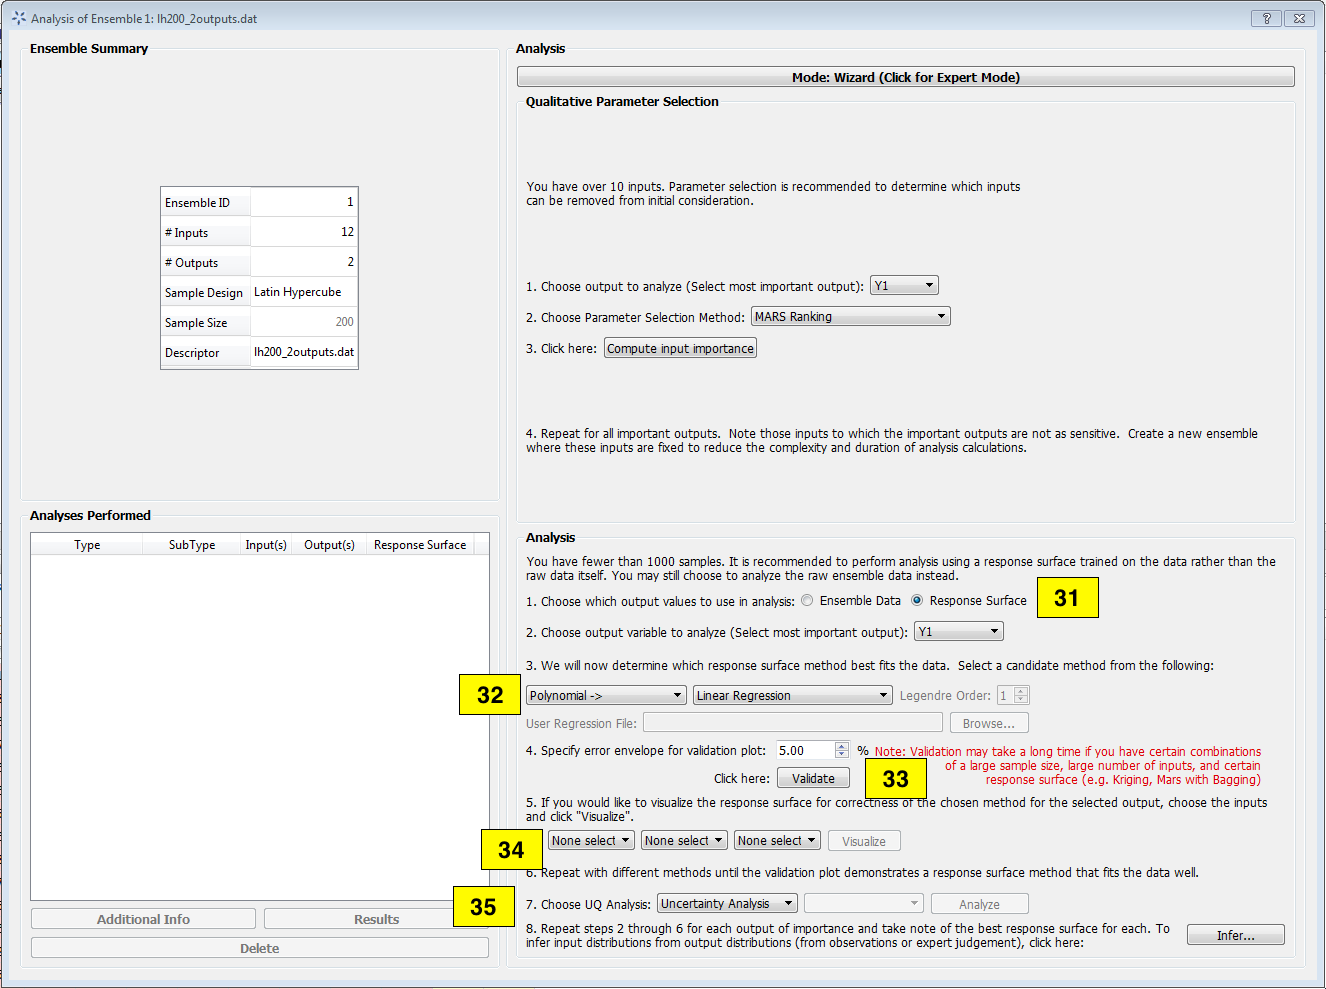
\includegraphics[width=6.5in,height=4in,keepaspectratio]{Chapt_uq/figs/overview/4_Analyze2}
		\caption{Analysis Dialog, Response Surface Analysis, Wizard Mode}
		\label{fig:uq_analysisW2}
	\end{figure}
	\label{itm:uq_analysis}
}
\item
	\bu{Response Surface} enables the user to perform all analyses related to
	response surfaces. A response surface is an approximation of the
	input-to-output relationship. This is an inexpensive way to approximate
	the values of outputs given different input values when the actual
	simulation of output values is computationally intensive. FOQUS uses the
	data (i.e., input-output samples) to fit a response surface scheme. The
	first step in this analysis is to select which output to analyze.
\item
	Select the \bu{Response Surface Model} to be used to approximate the
	input-to-output mapping. Selection of ``Polynomial'' or ``MARS''
	requires one further selection in the second drop-down list. If
	``Polynomial'' is chosen in the first drop-down list and ``Legendre'' is
	chosen in the second drop-down list, the user needs to specify a number for
	the \bu{Legendre polynomial order} before analysis can proceed.
	\label{itm:uq_rs}
\item
	The response surface selected must be validated before further analyses
	can be performed. The user can specify the error envelope for the validation plot. 
	When \bu{Validate} is clicked, the resulting plots display the best fit between the response 
	surface (based on the model selected) and the actual data.
\item
	\bu{Choose UQ Analysis} enables the user to perform
	response-surface-based UQ analyses. 
   Select the analysis in the first drop-down list. If the desired analysis is Sensitivity Analysis, select the desired type of sensitivity
	analysis in the second drop-down list and then
	click \bu{Analyze}. \textbf{\underline{Uncertainty Analysis}} and \textbf{\underline{Sensitivity Analysis}}
	compute and display the same quantities as in item
	\#\ref{itm:uq_analysis}. However, the results displayed are based on
	samples drawn from the trained response surface, not the simulation
	ensemble itself. Moreover, if the selected response surface has
	uncertainty, the resulting plots also reflect this uncertainty
	information.
\item
	FOQUS also provides visualization capabilities, enabling the user to 
   view the response surface as a function of one or multiple inputs. 
   Up to three inputs can be visualized at once. Click \bu{Visualize} to view. 
   %The threshold controls on the bottom
	%of the dialog enable the user to focus visualization on the subspace of
	%the output parameter that has values bounded by these thresholds. 
   A 2-D line plot displays if only one input parameter is selected. A 3-D
	surface plot and a 2-D contour plot display if two input parameters are
	selected. A 3-D isosurface plot with a slider bar displays if three
	input parameters are chosen. For the isosurface plot, the user can use
	the slider to selectively display the
	3-D input parameter space that activates a particular range in the
	output parameter. %%% TO DO: thresholds only exist in Expert mode now
\suspend{enumerate}

Finally, the \textbf{\underline{Bayesian Inference of Ensemble}} dialog (shown in Figure \ref{fig:uq_inf})
is used to calculate the posterior distributions (prior distributions
integrated with data) of the uncertain input parameters. 
%For each output variable, the user specifies an observed value (from
%physical experiments) with the associated uncertainties (in the form of
%standard deviations), if applicable. 
Inference utilizes Markov Chain Monte Carlo
(MCMC) to compute the posterior distributions, using response surfaces
that serve as fast approximations to the actual simulation model.


%%% INSERT Bayesian Inference Section
\begin{figure}[H]
\centering 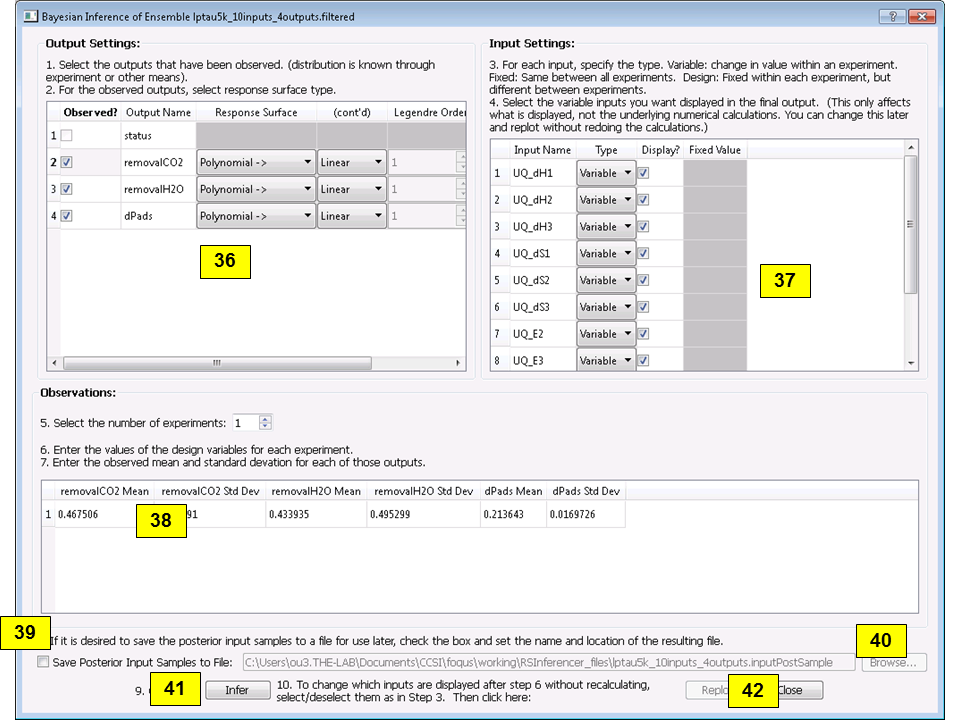
\includegraphics[width=6.5in,height=4in,keepaspectratio]{Chapt_uq/figs/overview/5_InferenceWizard2}
\caption{Bayesian Inference Dialog}
\label{fig:uq_inf}
\end{figure}
%%% TO DO: update section with design variables
\resume{enumerate}
\item
	Inference uses a response surface to approximate the
	input-to-output mapping. In \bu{Output Settings}, select the observed
	outputs and select the response surface type that works best with each
	observed output. As in item (\ref{itm:uq_rs}), further selections may be
	required based on	the response surface chosen. The simulation ensemble is used as the training data for
	generating the response surfaces.
\item
	The user can specify which inputs are fixed, design (fixed per
	experiment, but changes between experiments), or variable using
	the \bu{Input Settings Table}. In addition, the user can specify which
	inputs are displayed in the resulting plots of the posterior
	distributions. By default, once inference completes, all inputs will be
	displayed in the plots. To omit specific inputs, clear the checkboxes from
	the \textbf{\underline{Display}} column of the table.  
   Finally, in \textbf{\underline{Expert}} mode, this table can also be used to modify the input
	prior	distributions. The default prior is the input
	distribution specified in the simulation ensemble. 
   To change the prior distribution type, use the drop-down list in the \textbf{\underline{PDF}}
	column and enter corresponding values for the PDF parameters. 
   To change the range of a uniform prior, scroll all the way to the right
	to modify \textbf{\underline{Min/Max}}. 
\item
	The \bu{Observations} section enables the user to add experimental data
   in the form of observations of certain output variables.
   At least one observation is required.
   Currently, the	observation noise model is assumed to be a normal
	distribution. Other distributions may be supported in the future. To
	specify the observation noise model, enter the mean (and standard
	deviation, if standard inference is selected) for each output observation. For
	convenience, the \textbf{\underline{Mean}} and \textbf{\underline{Standard Deviation}} fields have been populated
	with the statistics from the ensemble uncertainty analysis. If any inputs
   are selected as design inputs, their values will also be required here.
\item
	\bu{Save Posterior Input Samples to File} checkbox, when selected, saves the
	posterior input samples as a PSUADE sample file	(format described in
	Section \ref{ap:psuadefiles}). This file characterizes the input
	uncertainty as a set of samples, which can be re-used in the \textbf{\underline{Simulation Ensemble
	Setup}} dialog, to evaluate the outputs corresponding to these posterior
	input samples.
\item
	If saving posterior samples to a file, click \bu{Browse} to set the
	name and location of where this file is saved.
\item
	Click \bu{Infer} to start the analysis. (Note: If the inference returns
	an invalid posterior distribution (i.e., one with no samples), it
	usually means the prior distributions or that the observation data
	distributions are not prescribed appropriately. In this case, it is
	recommended that the user experiment with different priors and/or data
	distribution means and/or standard deviations.)
\item{Inference calculations often take a very long time. If inference has
	run to completion, use \bu{Replot} to generate new plots (e.g., to only
	display a subset of the input posterior graphs) from the cached
	inference results.}
\end{enumerate}

\subsection{Simulation Ensemble Setup Dialog}
\label{subsec:uq_simsetup}

The \textbf{\underline{Simulation Ensemble Setup}} dialog (shown in Figure \ref{fig:uq_sim_dist}) is used
to create a new simulation ensemble. This is done by: (1) setting up
distribution parameters and generating samples, or (2) loading samples from
a file. This dialog is displayed when selecting \bu{Add New} on the UQ
window (Figure \ref{fig:uq_screen}).

%%% INSERT: Simulation Setup Dialog, Distributions Tab
\begin{figure}[H]
\centering 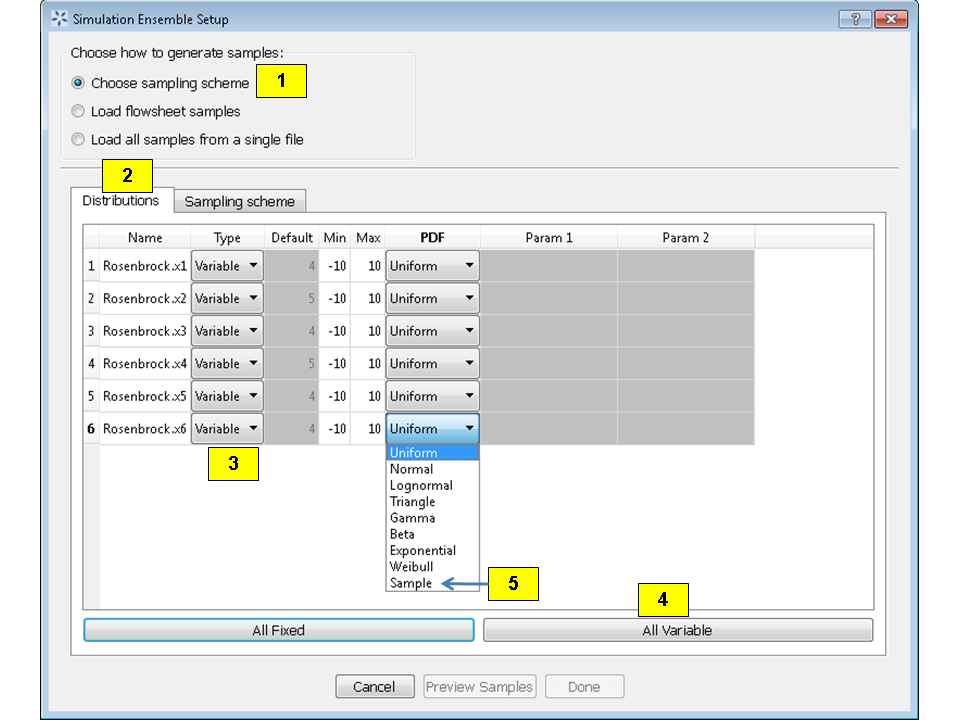
\includegraphics[width=6.5in,height=4in,keepaspectratio]{Chapt_uq/figs/overview/6_SimSetupDist2}
\caption{Simulation Ensemble Setup Dialog, Distributions Tab}
\label{fig:uq_sim_dist}
\end{figure}

\begin{enumerate}
\item
	Choose how to generate samples. There are three options:
	(1) \bu{Choose sampling scheme} (default), (2) \bu{Load flowsheet
	samples}, or (3) \bu{Load all samples from a single file}. The option 3
	is explained in item (\ref{itm:uq_sim_last}). 
	\label{itm:uq_sim_first}
\item
	If \textbf{\underline{Choose Sampling Scheme}} is selected, the \bu{Distributions} tab is
	displayed. The user specifies the input uncertainty information.
\item
	The \bu{Distributions Table} is pre-populated with input variable
	information gathered from the flowsheet node. Under the \bu{Type} column drop-down list, the user can select ``Fixed'' or ``Variable''. Selecting ``Fixed'' means that the input is fixed at its
	default value for all the samples. Changing the type to ``Variable''
	means that the input is uncertain; therefore, its value varies between
	samples. With any fixed input, the only parameter that can be changed is
	the \textbf{\underline{Default}} value (i.e., all samples of this input are fixed at this
	default value). With any variable input, the \textbf{\underline{Min/Max}} values, as
	well as the probability distribution function (\textbf{\underline{PDF}}), for that input can
	be changed. Some PDFs have their own parameters (e.g., mean and standard
	deviation for a normal distribution), which are required in the
	columns right of the distribution column. See the PSUADE manual for more
	details on the different PDFs.
\item
	\bu{All Fixed} and \bu{All Variable} are convenient ways to set all the
	inputs to variable or fixed.
\item
	Note: A ``Sample'' PDF refers to sampling with replacement (i.e., input
	samples would be randomly drawn, with replacement, from a sample file). 
   If the selected distribution for any input is ``Sample'', then
   the following parameters are required: (1) the path of the sample
	file (which must conform to the sample format specified in
	Section \ref{ap:psuadefiles}); (2) the output index that designates which
	output is to be used. 
\item
	In the \bu{Sampling scheme} tab (Figure \ref{fig:uq_sim_samplescheme}),
	specify the sampling scheme, the sample size, and perform sample
	generation.
	%%% INSERT: Simulation Setup Dialog, Sampling Scheme Tab
	\begin{figure}[H]
		\centering 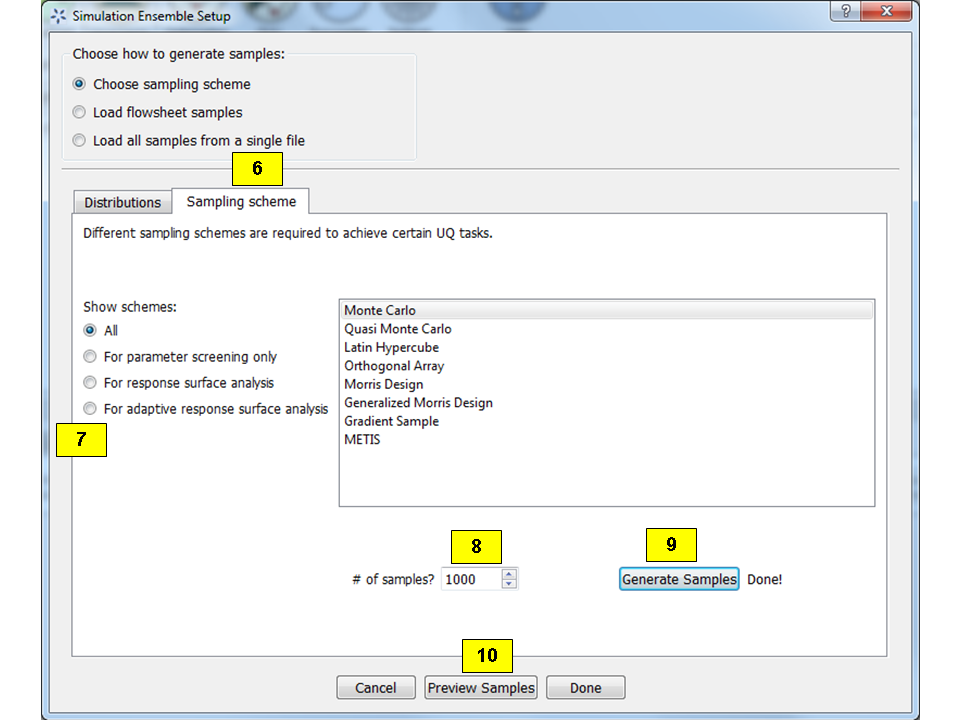
\includegraphics[width=6.5in,height=4in,keepaspectratio]{Chapt_uq/figs/overview/7_SimSetupSchemes2}
		\caption{Simulation Ensemble Setup Dialog, Sampling Scheme Tab}
		\label{fig:uq_sim_samplescheme}
	\end{figure}
\item
	Each radio button displays a different list of sampling schemes on the
	right. The radio buttons serve as a guide to help in the selection of
	the appropriate sampling schemes for target analyses. 
   A sampling scheme must be selected from the list on the right
	to proceed.
\item
	Set the number of samples to be generated from the \bu{\# of samples} spinbox.
\item
	When all parameters are set, click \bu{Generate Samples}. This generates
	the values for all the input variables, based on the sampling scheme selected.
\item
	Once samples have been generated, click \bu{Preview Samples} to view the
	samples that were generated. This displays the sample values in table
	form, as well as graphically as a scatter plot.
\item
	From item (\ref{itm:uq_sim_first}), if the user elects to load all
	samples from a single file, click \bu{Browse} to select the file
	containing the samples (Figure \ref{fig:uq_sim_loadsample}). This file
	must conform to the PSUADE full file format, the PSUADE sample format, or CSV file
	(all formats described in Section \ref{ap:psuadefiles}). Note: This is
	the only place where all the formats are supported. Once the file is
	loaded, the file name displays in the text box. These samples can now
	be used in the same way as an ensemble that was newly generated (as
	described above).
	%%% INSERT: Simulation Setup Dialog, Load Samples Screen
	\begin{figure}[H]
		\centering \includegraphics[width=6.5in,height=4in,keepaspectratio]{Chapt_uq/figs/overview/8_SimSetupLoad2}
		\caption{Simulation Ensemble Setup Dialog, Load Samples Option}
		\label{fig:uq_sim_loadsample}
		\end{figure}
		\label{itm:uq_sim_last}
\end{enumerate}
